\documentclass[14pt, a4paper]{article}
\usepackage{minitoc}
\usepackage[left=3.00cm, right=2.5cm, top=2.00cm, bottom=2.00cm]{geometry}
\usepackage{amsmath}
\usepackage{amssymb}
\usepackage{amsthm}
\usepackage{mathtools}
\usepackage{graphicx}
%\usepackage{algpseudocode}
%\usepackage{algorithm}
\usepackage[ruled,vlined,linesnumbered]{algorithm2e}
\usepackage{blindtext}
\usepackage{setspace}
\usepackage[utf8]{inputenc}
\usepackage[utf8]{vietnam}
\usepackage[center]{caption}
\usepackage[shortlabels]{enumitem}
\usepackage{fancyhdr} % header, footer
\usepackage{hyperref} % loại bỏ border với mục lục và công thức
\usepackage[nonumberlist, nopostdot, nogroupskip]{glossaries}
\usepackage{glossary-superragged}
\usepackage{tikz,tkz-tab}
\usepackage{pythonhighlight}
\setglossarystyle{superraggedheaderborder}
\pagestyle{fancy}
%\usepackage[style=numeric,sortcites]{biblatex}
%\addbibresource{ref.bib}
%\usepackage[numbers]{natbib}
\usepackage{indentfirst}
\usepackage[natbib,backend=biber,style=ieee, sorting=ynt]{biblatex}

\usepackage{caption}
\usepackage{subcaption}

\bibliography{ref.bib}

\graphicspath{{./figures/}}

\fancyhf{}
%\rhead{\textbf{Môn học: Các phương pháp thống kê hiện đại trong nghiên cứu Xã hội học}}
\lhead{\textbf{GVHD: TS. Trịnh Quốc Anh}}
\rfoot{\thepage}
\lfoot{\textbf{Học viên thực hiện: Nguyễn Chí Thanh - 21007925}}
\renewcommand{\headrulewidth}{0.4pt}
\renewcommand{\footrulewidth}{0.4pt}
%
%\numberwithin{equation}{section}
%\numberwithin{algorithm}{section}
%\numberwithin{figure}{section}
%
%\setlength{\parindent}{0.5cm}
%
%\setcounter{secnumdepth}{3} % Cho phép subsubsection trong report
%\setcounter{tocdepth}{3} % Chèn subsubsection vào bảng mục lục

%\newtheorem{dl}{Định lý}
%\newtheorem{md}{Mệnh đề}
%\newtheorem{bd}{Bổ đề}
%\newtheorem{dn}{Định nghĩa}
%\newtheorem{hq}{Hệ quả}

%\newtheorem{baitap}{Bài tập}
%\newtheorem*{loigiai}{Lời giải}

%\numberwithin{dl}{section}
%\numberwithin{md}{section}
%\numberwithin{bd}{section}
%\numberwithin{dn}{section}
%\numberwithin{hq}{section}

\setlength{\parindent}{0cm}

\newtheorem{dl}{Định lý}
\newtheoremstyle{sltheorem}
{}                % Space above
{}                % Space below
{\normalfont}        % Theorem body font % (default is "\upshape")
{}                % Indent amount
{\bfseries}       % Theorem head font % (default is \mdseries)
{.}               % Punctuation after theorem head % default: no punctuation
{ }               % Space after theorem head
{}                % Theorem head spec
\theoremstyle{sltheorem}
\newtheorem{baitap}{Bài tập}
\newtheoremstyle{soltheorem}
{}                % Space above
{}                % Space below
{\normalfont}        % Theorem body font % (default is "\upshape")
{}                % Indent amount
{\bfseries}       % Theorem head font % (default is \mdseries)
{.}               % Punctuation after theorem head % default: no punctuation
{\newline}               % Space after theorem head
{}                % Theorem head spec
\theoremstyle{soltheorem}
\newtheorem*{loigiai}{Lời giải}

\onehalfspacing

\begin{document}
\begin{titlepage}

    \newcommand{\HRule}{\rule{\linewidth}{0.5mm}} % Defines a new command for the horizontal lines, change thickness here

    \center % Center everything on the page

    %----------------------------------------------------------------------------------------
    %	HEADING SECTIONS
    %----------------------------------------------------------------------------------------
    \textsc{\LARGE Đại học Quốc Gia Hà Nội}\\[0.5cm]
    \textsc{\LARGE Trường đại học Khoa học tự nhiên}\\[0.5cm] % Name of your university/college
    \textsc{\LARGE Khoa Toán - Cơ - Tin học}\\[0.5cm]

    
\includegraphics[scale=0.2]{HUS-logo.jpg}\\[0.5cm]

    \textsc{\Large Chuyên ngành: Khoa học dữ liệu}\\[0.5cm] % Major heading such as course name


    %----------------------------------------------------------------------------------------
    %	TITLE SECTION
    %----------------------------------------------------------------------------------------

    \HRule \\[0.4cm]
    { \huge \bfseries Bài tập môn học}\\[0.4cm] % Title of your document
    \HRule \\[1.5cm]

    \textsc{\Large Môn học: Các phương pháp thống kê hiện đại \\ trong nghiên cứu Xã hội học}\\[1cm] % Minor heading such as course title


    \textsc{\Large Bài tập số 4}\\[1cm]


    %----------------------------------------------------------------------------------------
    %	AUTHOR SECTION
    %----------------------------------------------------------------------------------------
    \begin{minipage}{0.4\textwidth}
        \begin{flushleft} \large
        \emph{Giảng viên hướng dẫn:} \\
        TS. Trịnh Quốc Anh % Supervisor's Name
        \end{flushleft}
    \end{minipage}\\[0.5cm]

    \begin{minipage}{0.4\textwidth}
    \begin{flushleft} \large
    \emph{Học viên thực hiện:}\\
    Nguyễn Chí Thanh \\
    MSHV: 21007925 \\ % Your name
    Lớp: Khoa học dữ liệu - K4
    \end{flushleft}
    \end{minipage}


    % If you don't want a supervisor, uncomment the two lines below and remove the section above
    %\Large \emph{Author:}\\
    %John \textsc{Smith}\\[3cm] % Your name

    %----------------------------------------------------------------------------------------
    %	DATE SECTION
    %----------------------------------------------------------------------------------------

    % I don't want day because it is English
    % {\large \today}\\[2cm] % Date, change the \today to a set date if you want to be precise

    %----------------------------------------------------------------------------------------
    %	LOGO SECTION
    %----------------------------------------------------------------------------------------

    %\includegraphics{logo/rsz_3logo-khtn.png}\\[1cm] % Include a department/university logo - this will require the graphicx package

    %----------------------------------------------------------------------------------------

    \vfill % Fill the rest of the page with whitespace

\end{titlepage}

\nocite{*}

\newpage

\begin{baitap}
    Hãy tóm tắt về nghiên cứu "Who plays video games?":
    \begin{itemize}
        \item Vấn đề/câu hỏi cần nghiên cứu
        \item Dữ liệu dùng để nghiên cứu
        \item Cơ sở và phương pháp nghiên cứu
    \end{itemize}
\end{baitap}

\begin{loigiai}
    Hãy tóm tắt về nghiên cứu "Who plays video games?":
    \begin{itemize}
        \item Vấn đề/câu hỏi cần nghiên cứu:
        \begin{enumerate}
            \item Bắt đầu bằng cách đưa ra tỷ lệ sinh viên chơi game trong tuần trước khi cuộc khỏa sát diễn ra.
            Ước lượng khoảng tin cậy cũng như ước lượng điểm cho tỷ lệ này.
            \item Xét thời gian chơi gam trong tuần trước khi cuộc khảo sát diễn ra so với tần suất chơi ghi nhận được (hàng ngày, hàng tuần,...).
            Liệu nếu có một bài kiểm tra vào tuần trước khi diễn ra cuộc khảo sát có làm ảnh hưởng đến ước lượng ở câu hỏi trước?
            \item Tìm khoảng tin cậy cho thời gian chơi game trung bình của một sinh viên trước cuộc khảo sát.
            Ta cần chú ý đến phân phối mẫu.
            \item Ta xét về các câu hỏi mang tính "thái độ".
            Nhìn chung sinh viên có thích chơi gam hay không?
            Nếu ta phải lập một danh sách ngắn các lý do quan trọng vì sao sinh viên thích (hoặc không thích) chơi game, ta sẽ đưa gì vào danh sách?
            \item Tìm sự khác biệt giữa những sinh viên chơi game và những sinh viên không chơi game.
            Để làm được điều này, hãy sử dụng những câu hỏi trong phần cuối của cuộc khỏa sát và so sánh giữa sinh viên nam và sinh viên nữ,
            những người có đi hay làm hay không, có máy tính hay không hoặc những người đặt kỳ vọng được điểm A trong các môn học hay không.
            Một số phương pháp trực quan hữu ích trong so sánh các tiêu chí trên.
            \item Ta sẽ nghiên cứu sau hơn về điểm số mà các sinh viên mong muốn trong các môn học.
            Kết quả cuộc khảo sát với phù hợp với phân phối điểm là 20\% điểm A, 30 \% điểm B, 40 \% điểm C, 10 \% điểm D hoặc thấp hơn.
            Nếu những sinh viên không trả lời là những sinh viên bị trượt thì bức tranh toàn cảnh của cuộc khảo sát sẽ thay đổi thế nào?
        \end{enumerate}

        \item Dữ liệu dùng để nghiên cứu:
        
        95 trong tổng số 314 sinh viên tham gia khóa học Thống kê 2 vào mùa đông 1994 được chọn ngẫu nhiên tham gia vào cuộc khảo sát.
        Các câu hỏi đã được hoàn thành thu được từ 91 trong tổng số 95 sinh viên.
        Dữ liệu có được là các phản hồi của sinh viên đối với bảng câu hỏi.

        Cuộc khảo sát yêu cầu sinh viên xác định tần suất chơi game và điều gì làm sinh viên thích và không thích về các tựa game.
        Câu trả lời cho những câu hỏi này đã được mã hóa bằng số như được mô tả trong Bảng 2.1.
        Bảng 2.1 cũng cung cấp một vài mẫu quan sát. Nếu một câu hỏi không được trả lời hoặc trả lời không chính xác, thì nó được mã hóa thành 99. Tất cả các câu hỏi có câu trả lời có/không đều được ghi 1 cho "Có" và 0 cho "Không".
        Những người trả lời chưa bao giờ chơi game hoặc hoàn toàn không thích chơi game được yêu cầu bỏ qua nhiều câu hỏi.

        Cuộc khảo sát có thể tạm chia thành ba phần. Hai trong số ba phần liên quan đến việc chơi gam của sinh viên.
        Một trong những phần này xác định tần suất chơi game của sinh viên.
        Thông tin này được yêu cầu qua hai câu hỏi.
        Một câu hỏi hỏi sinh viên dành bao nhiêu thời gian chơi game vào tuần tước khi diễn ra khảo sát và câu hỏi còn lại hỏi tần suất chơi game của sinh viên (hàng ngày, hàng tuần, hàng tháng, học kỳ).

        Phân thứ hai của cuộc khảo sát bao gồm việc sinh viên có thích chơi game hay không và vì sao.
        Một bản tổng hợp các phản hồi cho ba trong số những câu hỏi này xuất hiện trong bảng 2.2,  2.3 và 2.4.
        Những câu hỏi này khác với những câu hỏi khác ở chỗ có thể đưa ra nhiều hơn một câu trả lời.
        Bảng 2.2 tóm tắc các thể loại game đã được sinh viên chơi.
        Sinh viên được yêu cầu đánh dấu vào tất cả các thể loại game mà sinh viên đã chơi.
        Ví dụ, 50 \% sinh viên trả lời câu hỏi này nói rằng họ có chơi game thuộc thể loại hành động.
        Không phải tất cả các sinh viên đều trả lời câu hỏi này, vì mootjsoos sinh viên nói rằng họ chưa từng chơi game hoặc không hề thích chơi game sẽ được hướng dẫn bỏ qua các câu hỏi này.
        Những sinh viên đã trả lời câu hỏi này cũng được hỏi lý do vì sao họ chơi các game đó.
        Họ được yêu cầu chọn ba lý do. Phản hồi của các sinh viên được trình bày trong bảng 2.3,
        Cuối cùng, bảng 2.4 tóm tắt những điều mà sinh viên không thích về các tựa game đó.
        Tất cả các sinh viên được yêu cầu trả lời câu hỏi này và được chọn tối đa ba lý do không thích chơi game.

        Phần thứ ba của bảng câu hỏi là thu thập các thông tin cá nhân chung về sinh viên như là tuổi, giới tính.
        Các sinh viên cũng được hỏi họ có tài khoản email hay không, họ có thích hay ghét môn toán không, điểm số các môn học mà họ kỳ vọng.

        Ta có tổng 314 sinh viên. Để chọn ra 95 sinh viên cho nghiên cứu, mỗi sinh viên được đánh số từ 1 đến 314.
        Một bộ sinh số ngẫu nhiên chọn 95 số giữa 1 và 314.
        Các sinh viên tương ứng được chọn vào nghiên cứu.

        Để khuyến kích trả lời trung thực, thì thông tin của sinh viên sẽ được giữa bí mật.
        Mọi phiếu trả lời không được điền tên.

        Để hạn chế số phiếu không phản hồi, hệ thống thu thập dữ liệu gồm ba bước được triển khai.
        Người thu thập dữ liệu sẽ đến vào thứ ba và thứ năm nói về cuộc khảo sát sẽ được thực hiện.
        Sinh viên đã làm bài kiểm tra trước cuộc khảo sát và được trả kết quả trong tuần thực hiện khảo sát.
        
        Cuối cùng, để tăng độ chính xác của cuộc khảo sát, người thu thập dữ liệu sẽ phải khuyến khích sinh viên và cho biết sự đảm bảo về thông tin cá nhân.

        Các game được phân loại theo các thiết bị mà game được chạy và loại kỹ năng cần để chơi game.
        Với thiết bị, được chia thành ba loại cơ bản: arcade, console và máy tính cá nhân.
        Với thể loại, game được chia thành năm thể loại: hành động, phiêu lưu, mô phỏng, chiến thuật và nhập vai.

        Đa số các arcade game là các game thuộc thể loại game hành động mà yêu cầu sự linh hoạt của tay và mắt và không cần thời gian học lâu.
        Game chạy trên console có thể là hành động, phiêu lưu hoặc chiến thuật.
        Các game mô phỏng hoặc nhập vai hay được chơi trên máy tính cá nhâ.
        Các game này không phù hợp trên arcade hoặc console vì cần nhiều giờ chơi.
        Các thể loại game đều có thể chơi trên PC.

        \item Cơ sở và phương pháp nghiên cứu:
        Ta sẽ sử dụng phương pháp học không giám sát là phân cụm.
        Nhưng nếu để nguyên dữ liệu, các điểm dữ liệu có số chiều rất lớn.
        Để việc phân tích hiệu quả, ta sẽ giảm chiều dữ liệu và phân cụm các điểm dữ liệu trên không gian đã được giảm chiều.
        Ta sẽ gán các cụm là các nhãn giả với từng mẫu dữ liệu.
        Ta thực hiện huấn luyện một mô hình phân loại trên dữ liệu đã được giảm chiều dùng PCA và nhãn tương ứng với các cụm.
        Sau khi có được mô hình phân loại ta sẽ biển đổi các trọng số được huấn luyện từ không gian giảm chiều trở lại không gian các đặc trưng gốc từ đó ta xác định những yếu tố ảnh hưởng nhiều đến việc phân loại sinh viên theo khả năng chơi game.
        Ta có mã giả thực hiện PCA:

        \begin{algorithm}[h!]
            \DontPrintSemicolon
            \KwIn{Dữ liệu $\mathcal{D} \in \mathbb{R}^{N \times d}$, tỷ lệ thông tin giữ lại $\alpha$}

            $\bold{\mu} \gets \dfrac{1}{N} \sum_{i=1}^N \bold{x}_i$\;
            $\bold{Z} \gets \mathcal{D} - \bold{\mu}^T$\;
            $\bold{\Sigma} \gets \dfrac{1}{N}\bold{Z}^T \bold{Z}$\;
            Tính các trị riêng $\lambda_1, \lambda_2, \dots, \lambda_d$ và các vector riêng tương ứng $\bold{e}_1, \bold{e}_2, \dots, \bold{e}_d$\;
            $f(r) \gets \dfrac{\sum_{i=1}^r \lambda_i}{\sum_{j=1}^d \lambda_j}$\;
            Tìm $r$ nhỏ nhất sao cho $f(r) \geq \alpha$\;
            $\bold{U} \gets \begin{bmatrix} \bold{e}_1  & \bold{e}_2  & \dots  & \bold{e}_r \end{bmatrix}$\;
            $\mathcal{D}_r \gets \mathcal{D} \times \bold{U}$\;
            \Return{$\mathcal{D}_r$}\;
            \caption{Thuật toán thực hiện PCA}
        \end{algorithm}

        Với:

        \begin{equation*}
            \mathcal{D} = \begin{bmatrix}
                \bold{x}_1^T \\ \bold{x}_2 \\ \vdots \\ \bold{x}_N^T
            \end{bmatrix} \in \mathbb{R}^{N \times d}
        \end{equation*}
        và:

        \begin{equation*}
            \bold{U} = \begin{bmatrix}
                \bold{e}_1 & \bold{e}_2 & \dots & \bold{e}_r
            \end{bmatrix} \in \mathbb{R}^{d \times r}
        \end{equation*}

        Khi ta tìm được các trọng số được huấn luyện của mô hình phân loại là $\bold{W}_{PCA} \in \mathbb{R}^{\mathrm{c} \times r}$ ($c$ là số lớp).
        Ta tìm các trọng số trong không gian dữ liệu ban đầu là $\bold{W} \in \mathbb{R}^{\mathrm{c} \times d}$ bằng công thức $\bold{W} =   \bold{W}_{PCA} \times \bold{U}^T$.
    \end{itemize}
\end{loigiai}


\begin{baitap}
    Hãy đề xuất mô hình phân loại sinh viên và khả năng chơi games
\end{baitap}

\begin{loigiai}
    Ta sẽ thực hiện thống kê mô tả tập dữ liệu.

    \begin{figure}[h!]
        \centering
        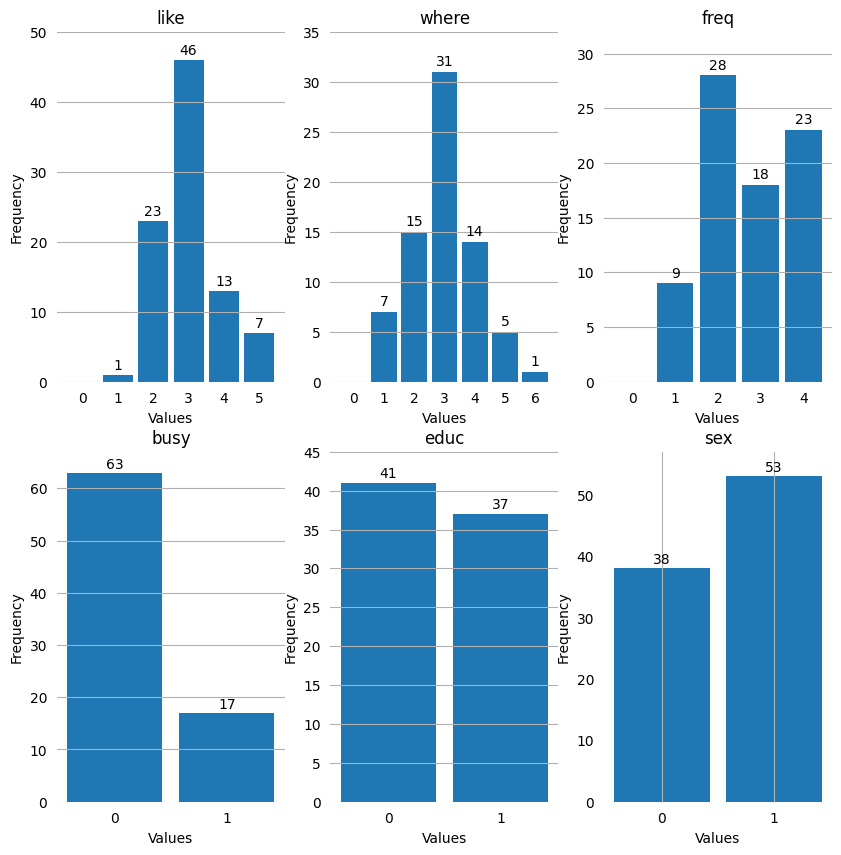
\includegraphics[width=0.6\textwidth]{1.png}
        \caption{Histogram của các trường like, where, freq, busy, educ, sex}
        \label{fig:1}
    \end{figure}

    \begin{figure}[h!]
        \centering
        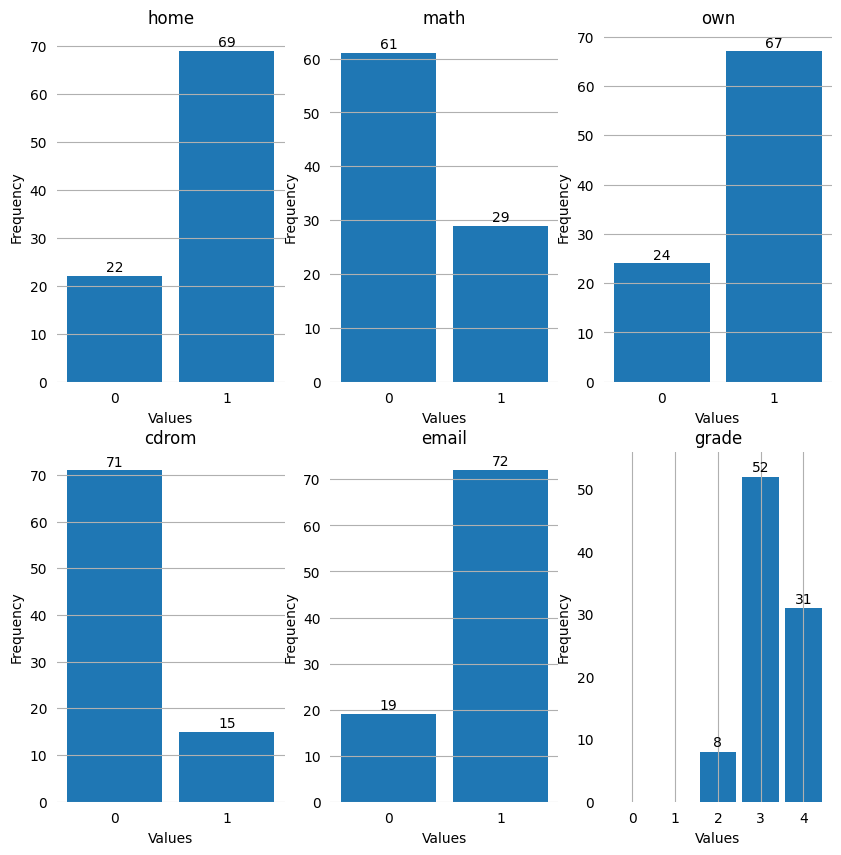
\includegraphics[width=0.6\textwidth]{2.png}
        \caption{Histogram của các trường home, math, own, cdrom, email, grade}
        \label{fig:2}
    \end{figure}

    \begin{figure}[h!]
        \centering
        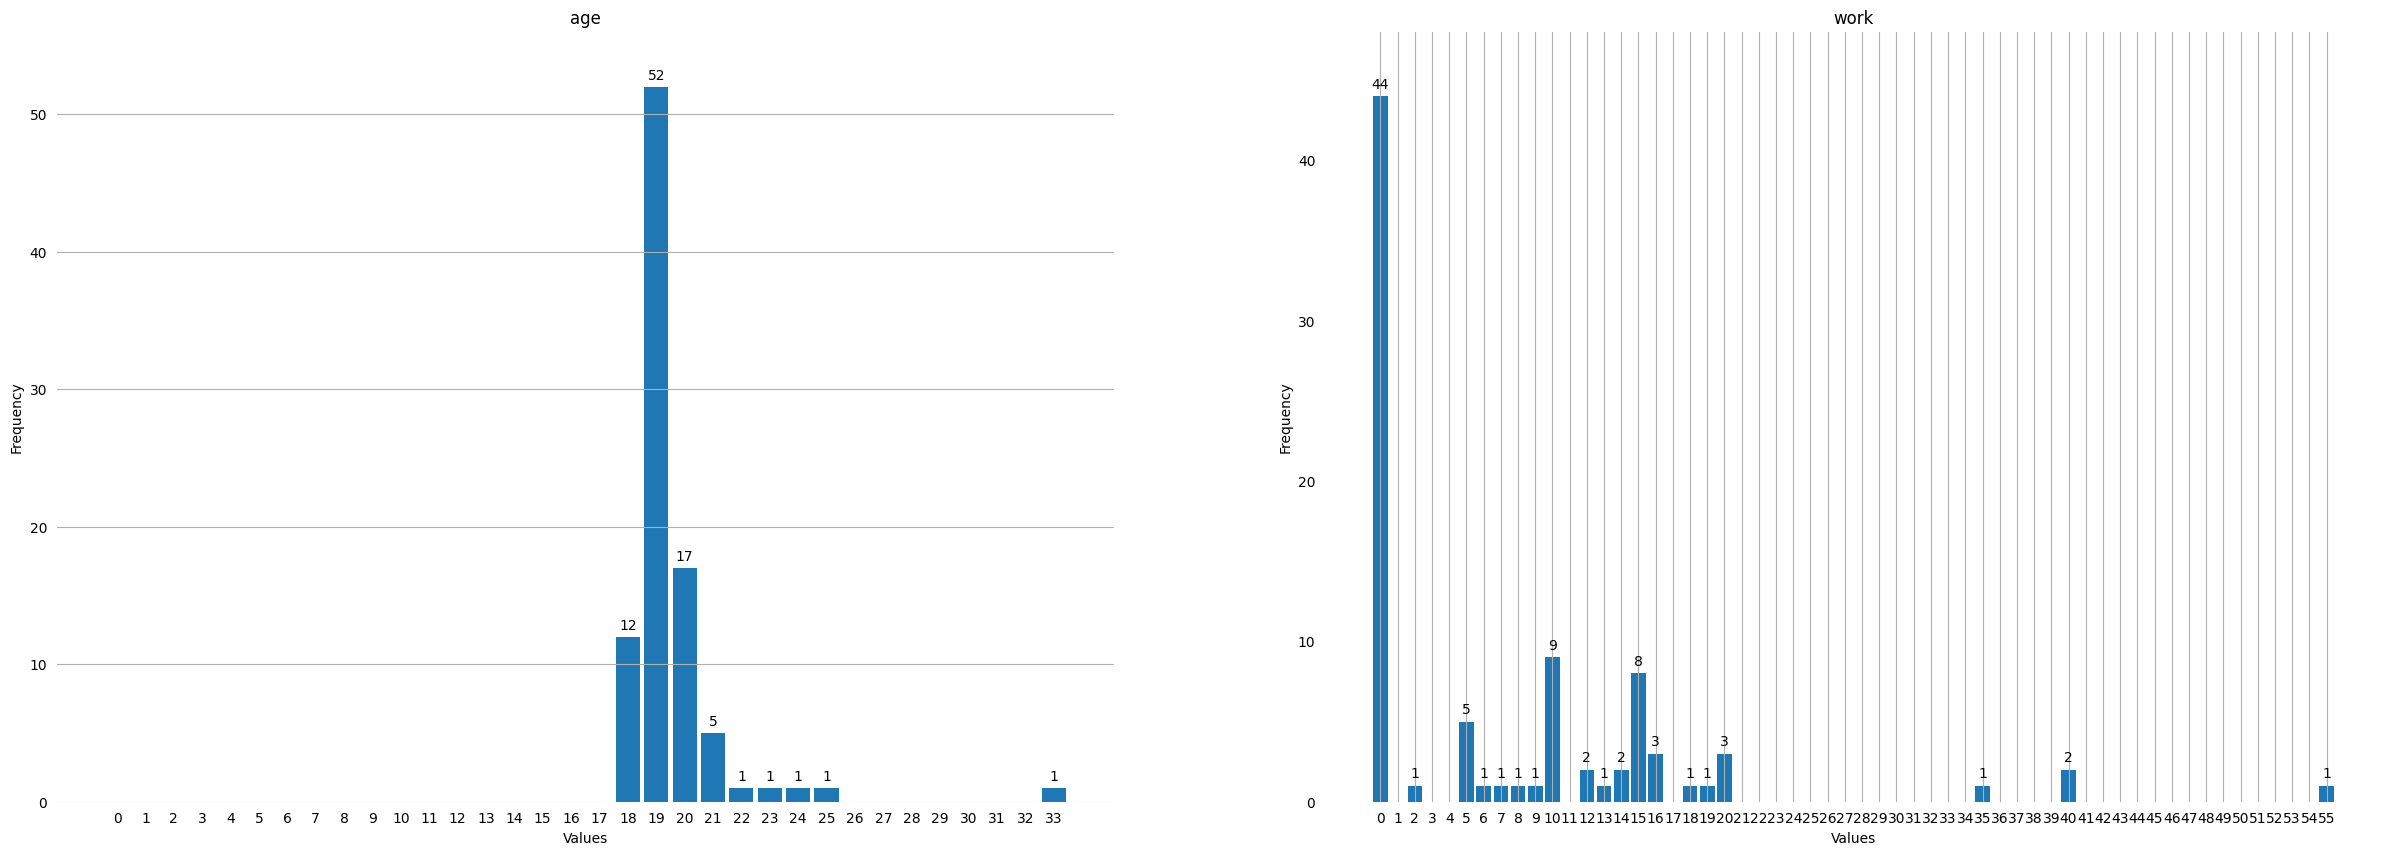
\includegraphics[width=0.6\textwidth]{3.png}
        \caption{Histogram của các trường age, work}
        \label{fig:3}
    \end{figure}

    \begin{figure}[h!]
        \centering
        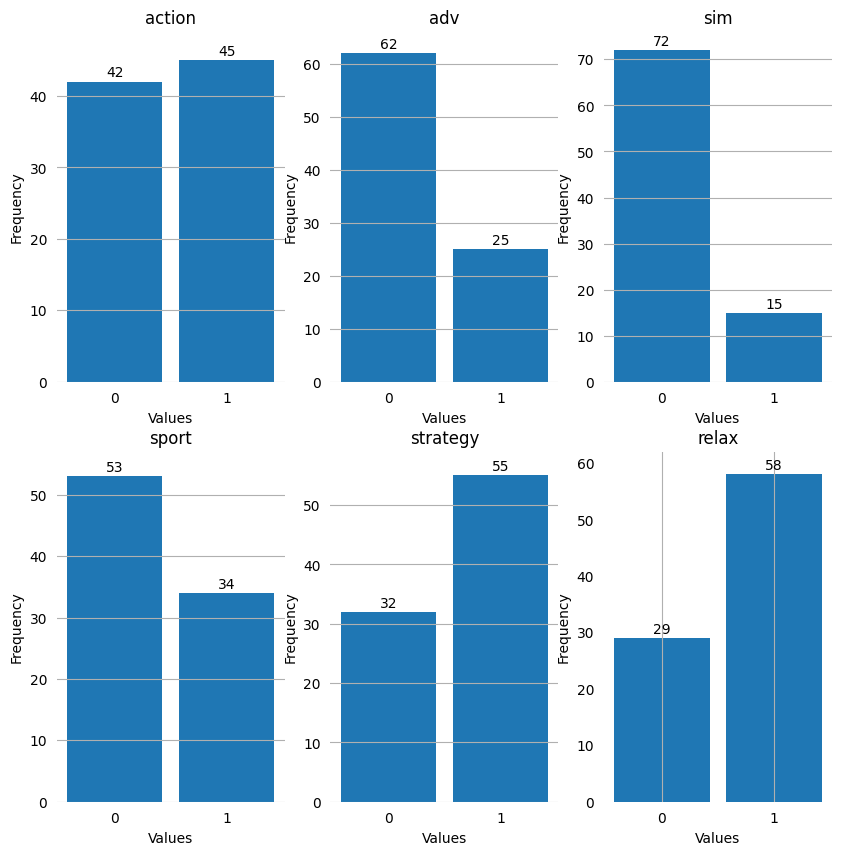
\includegraphics[width=0.6\textwidth]{4.png}
        \caption{Histogram của các trường action, adv, sim, sport, strategy, relax}
        \label{fig:4}
    \end{figure}

    \begin{figure}[h!]
        \centering
        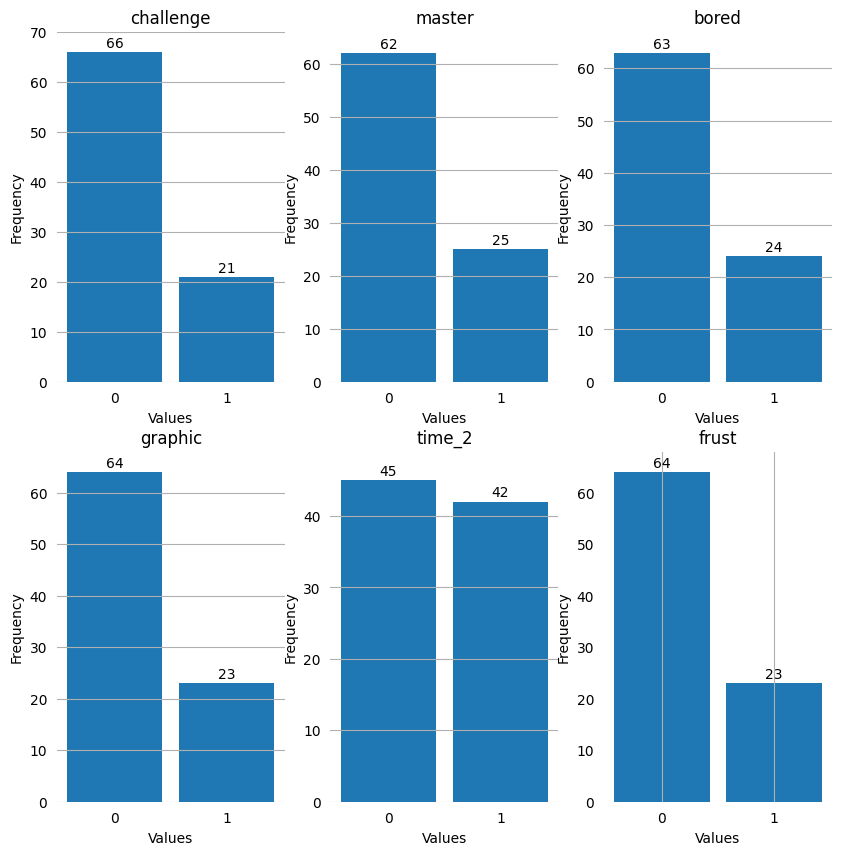
\includegraphics[width=0.6\textwidth]{5.png}
        \caption{Histogram của các trường challenge, master, bored, graphic, time\_2, frust}
        \label{fig:5}
    \end{figure}

    \begin{figure}[h!]
        \centering
        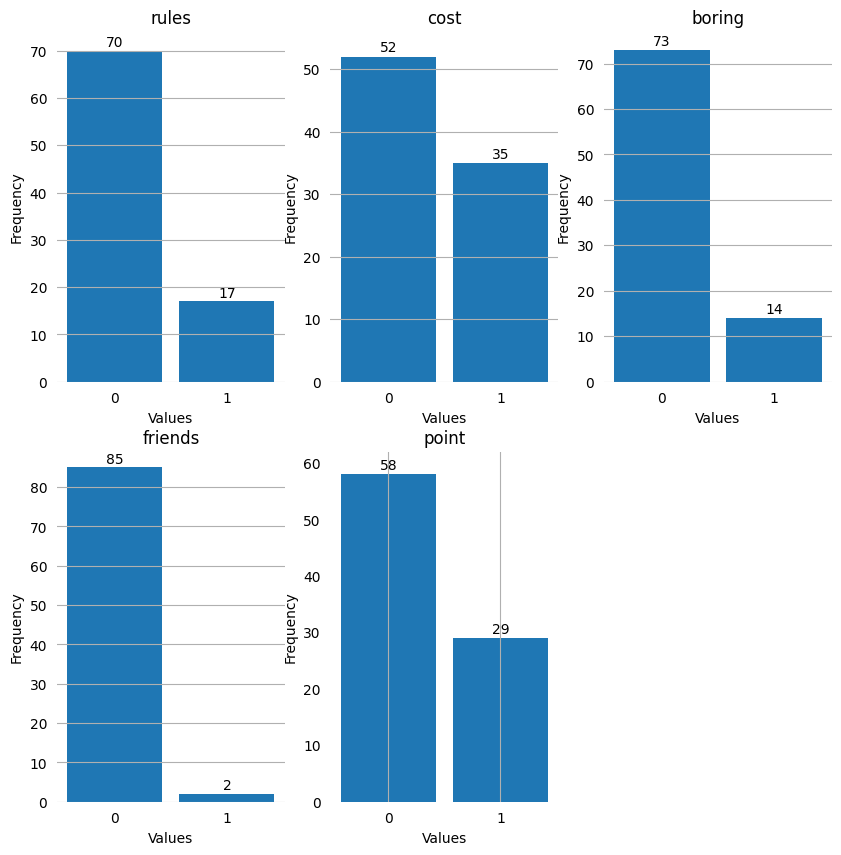
\includegraphics[width=0.6\textwidth]{6.png}
        \caption{Histogram của các trường rules, cost, boring, friends, points}
        \label{fig:6}
    \end{figure}

    \begin{figure}[h!]
        \centering
        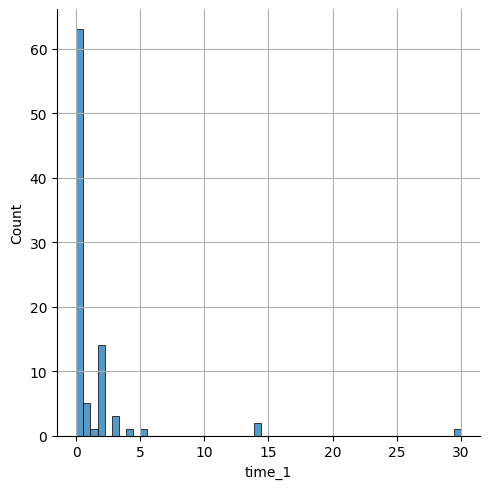
\includegraphics[width=0.6\textwidth]{7.png}
        \caption{Histogram của trường time\_1}
        \label{fig:7}
    \end{figure}

    \begin{figure}[h!]
        \centering
        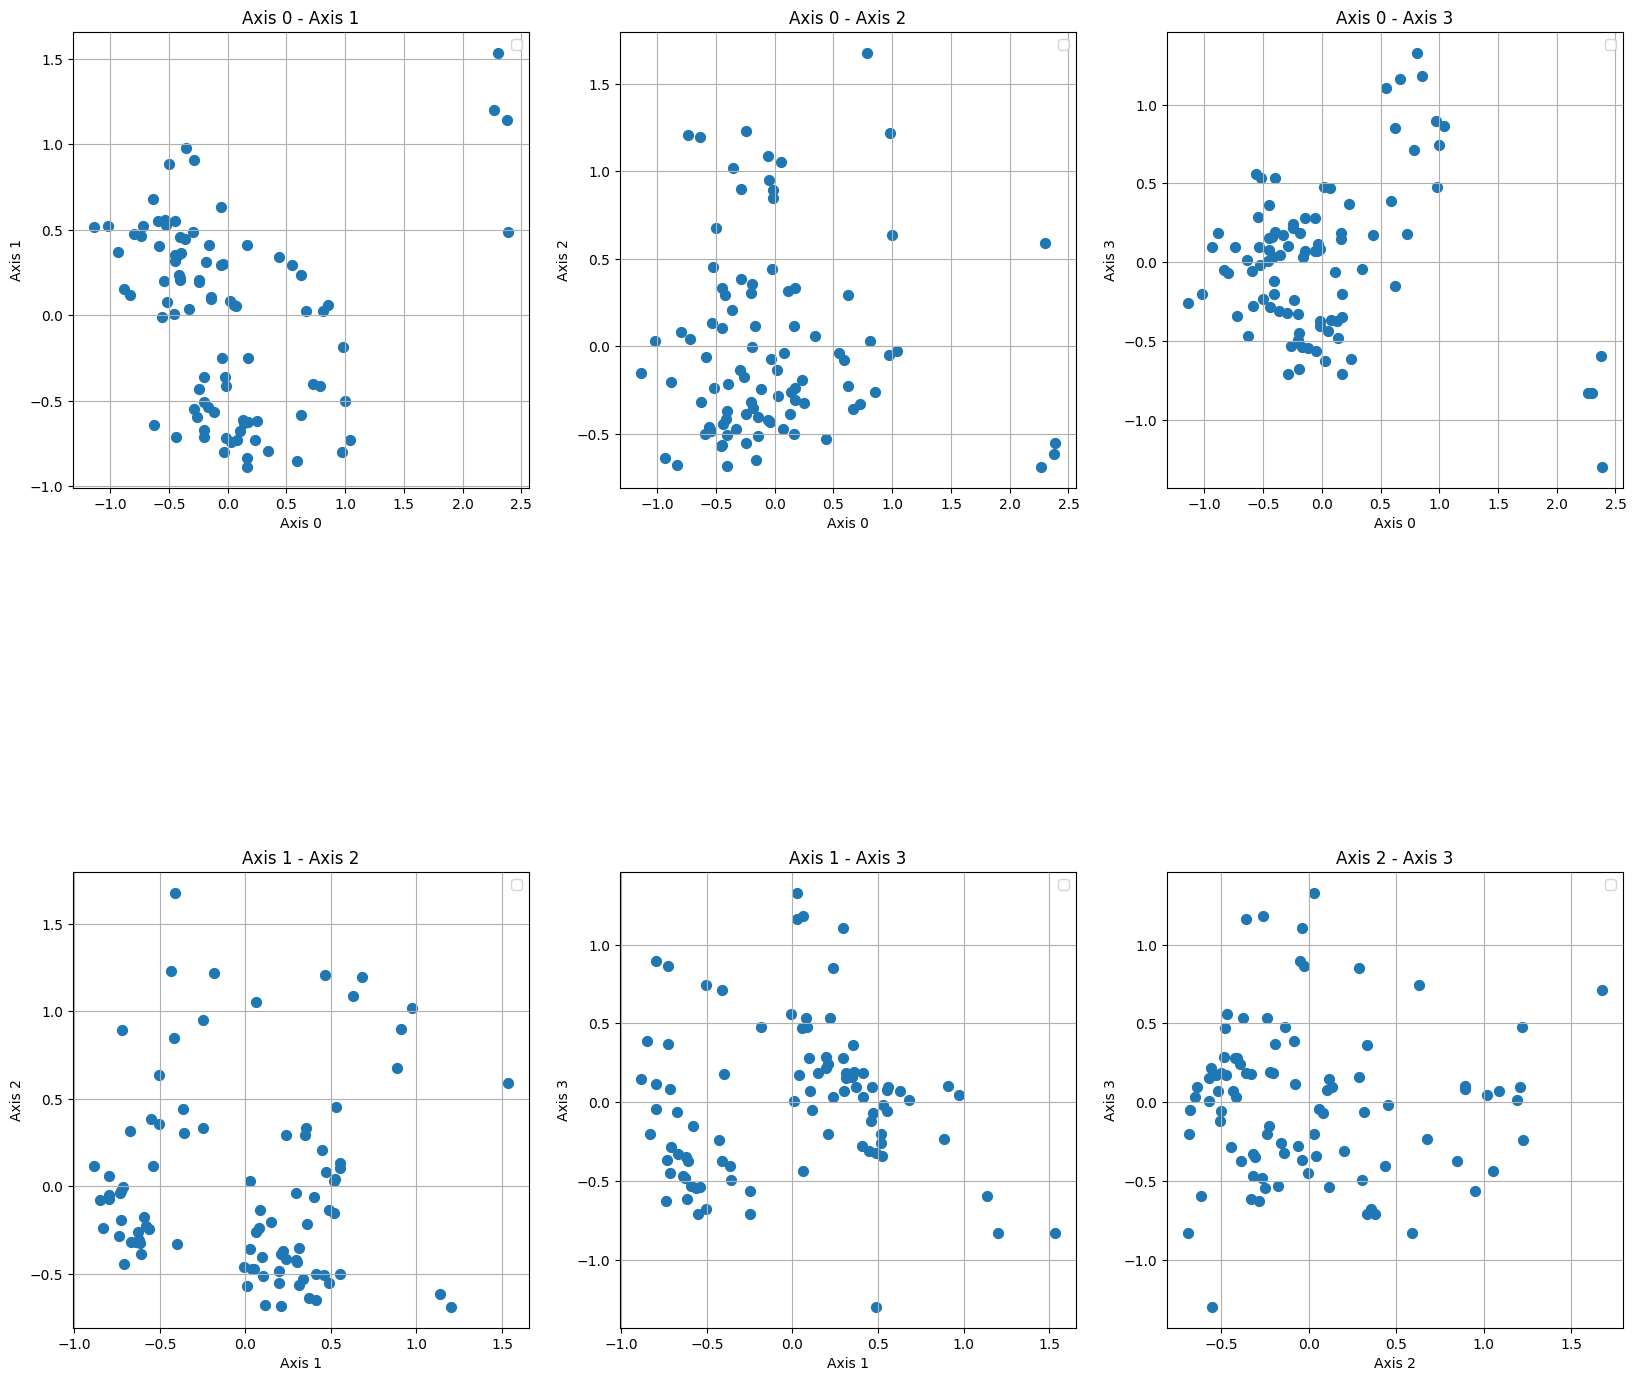
\includegraphics[width=0.75\textwidth]{figures/pca_scattering_4_dim.png}
        \caption{Scatter plot của các chiều thứ 0 đến chiều thứ 3 của dữ liệu sau khi được giảm chiều qua PCA}
        \label{fig:pca-scattering-4-dim}
    \end{figure}

    \begin{figure}[h!]
        \centering
        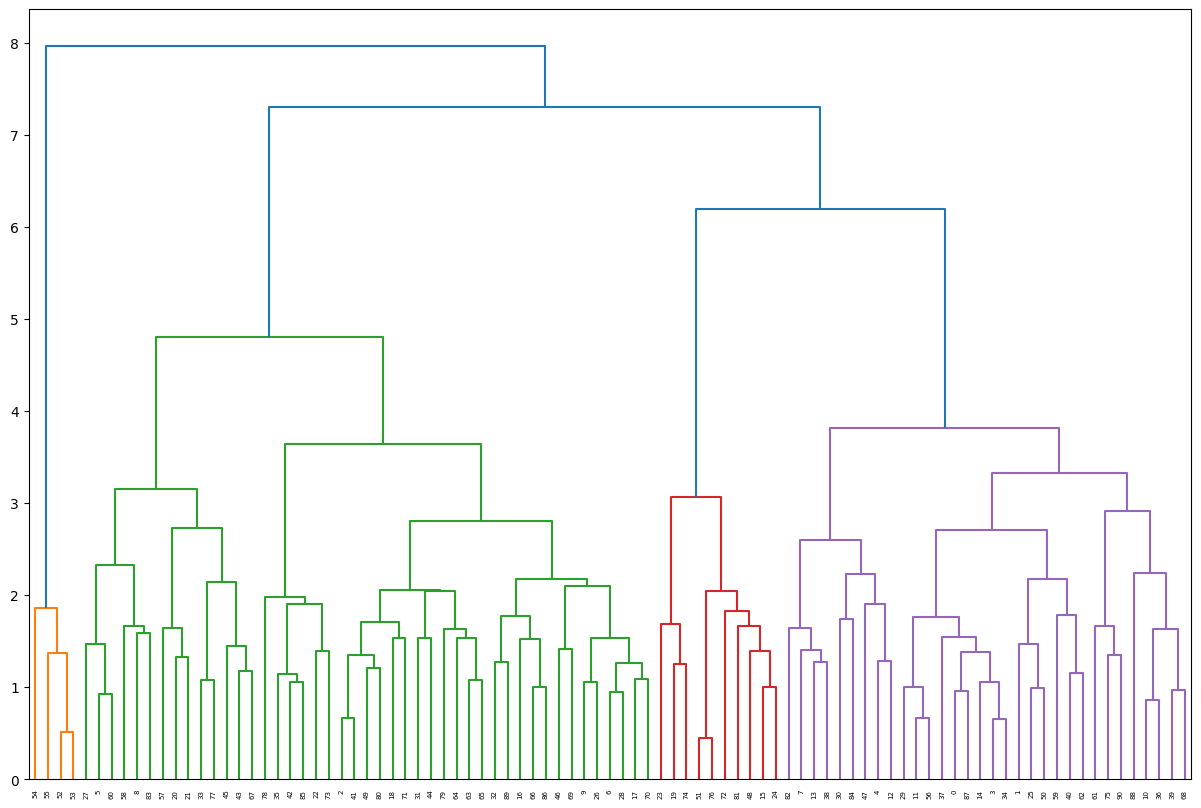
\includegraphics[width=0.6\textwidth]{figures/dendro_ward.png}
        \caption{Dendrogram được sử dụng dựa trên Ward linkage}
        \label{fig:dendro-ward}
    \end{figure}

    \begin{figure}[h!]
        \centering
        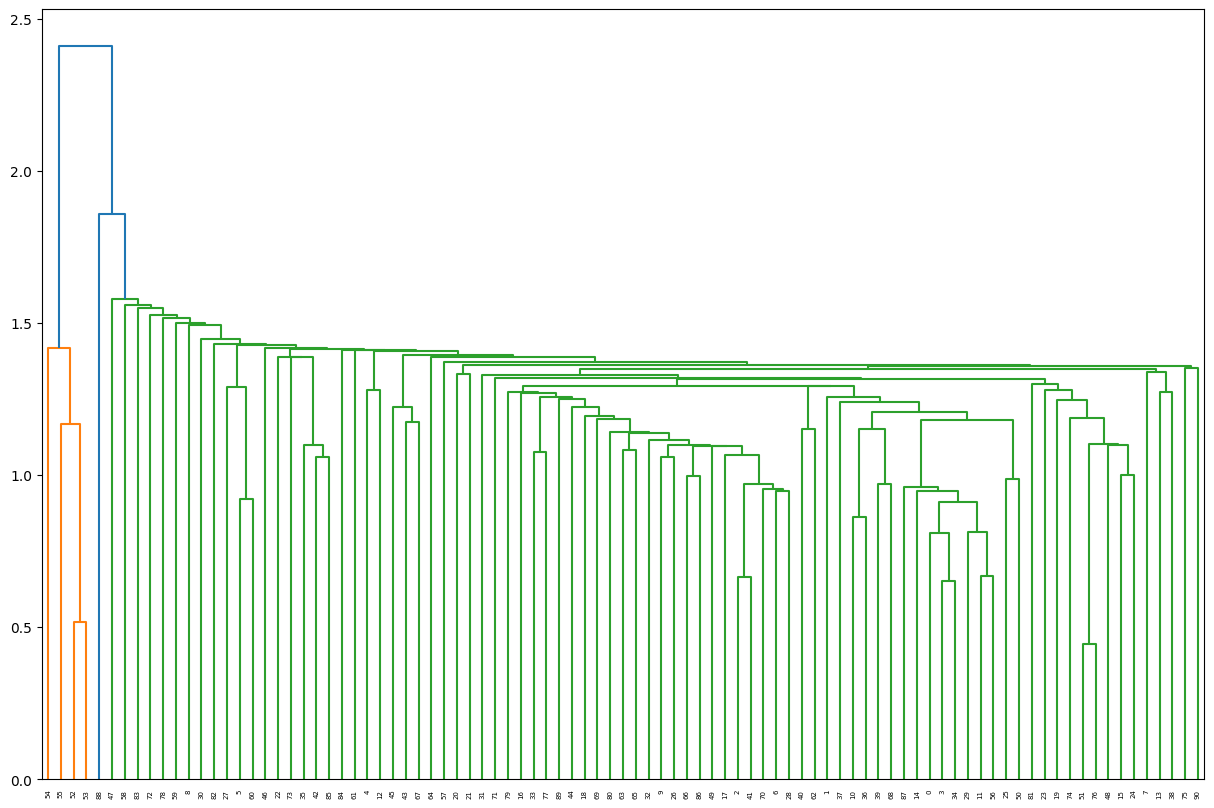
\includegraphics[width=0.6\textwidth]{figures/dendro_single.png}
        \caption{Dendrogram được sử dụng dựa trên Single linkage}
        \label{fig:dendro-single}
    \end{figure}

    \begin{figure}[h!]
        \centering
        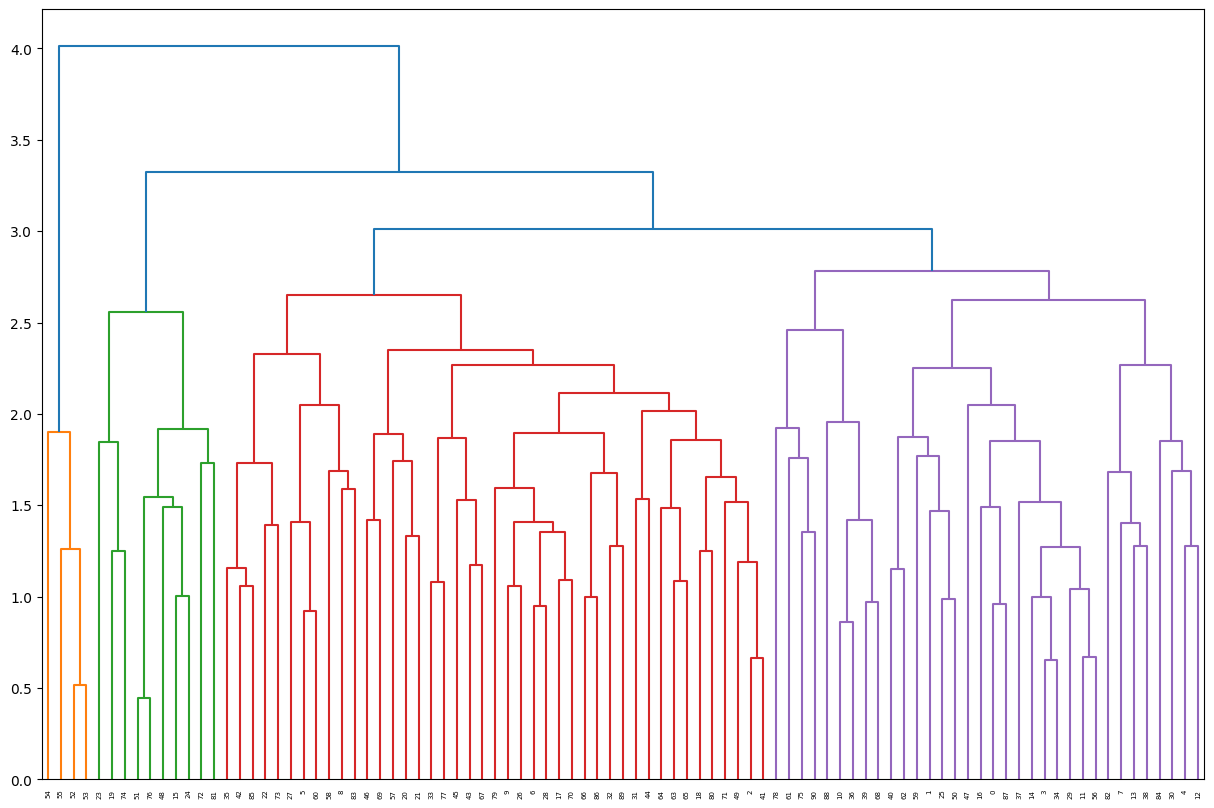
\includegraphics[width=0.6\textwidth]{figures/dendro_complete.png}
        \caption{Dendrogram được sử dụng dựa trên Complete linkage}
        \label{fig:dendro-complete}
    \end{figure}

    \begin{figure}[h!]
        \centering
        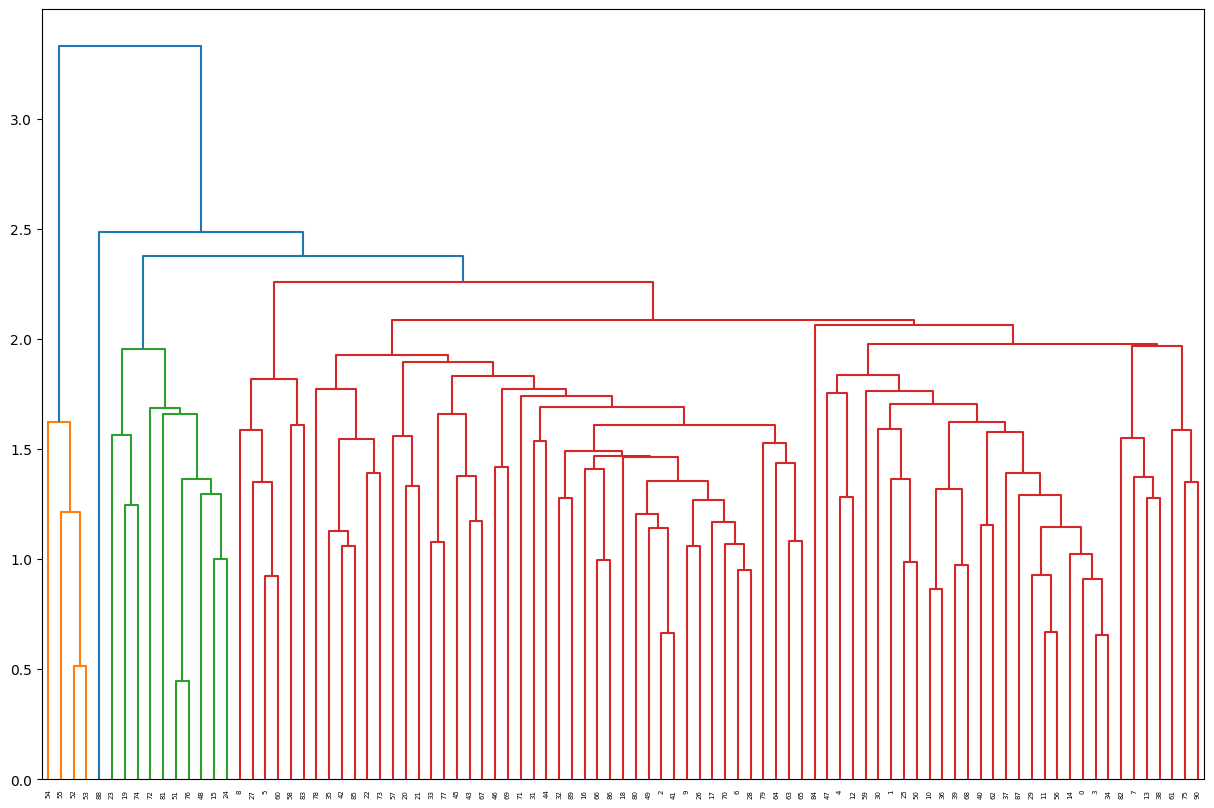
\includegraphics[width=0.6\textwidth]{figures/dendro_average.png}
        \caption{Dendrogram được sử dụng dựa trên Average linkage}
        \label{fig:dendro-average}
    \end{figure}

    \begin{figure}[h!]
        \centering
        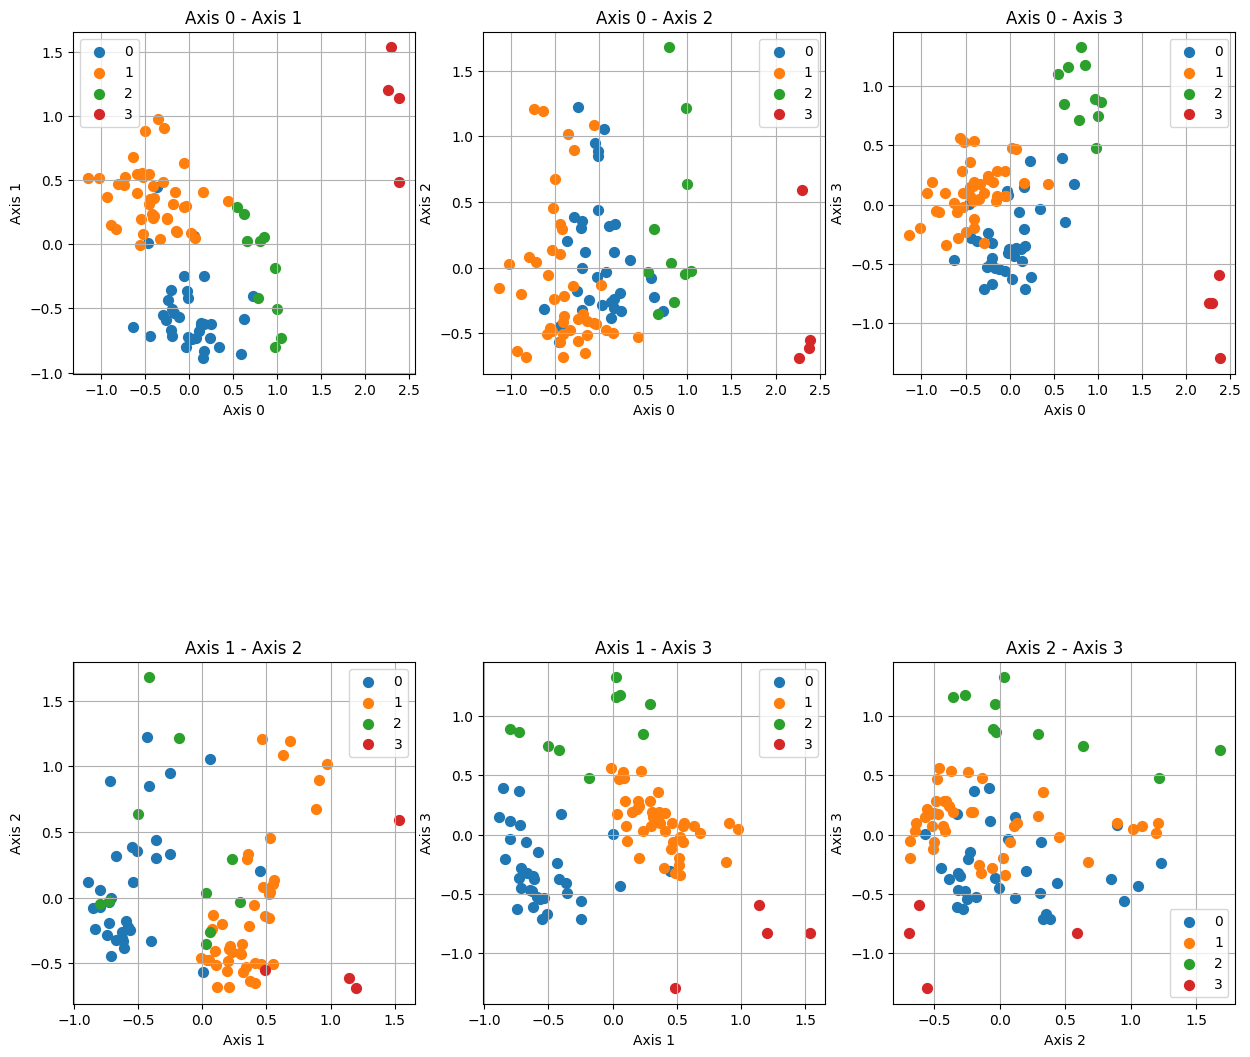
\includegraphics[width=0.75\textwidth]{figures/pca_scattering_4_dim_clustering.png}
        \caption{Scatter plot của các chiều thứ 0 đến chiều thứ 3 của dữ liệu sau khi được giảm chiều qua PCA và màu sắc tương ứng với các cụm được gán sau thuật toán Agglomerative Clustering}
        \label{fig:pca-scattering-4-dim-clustering}
    \end{figure}

    \begin{python}
clustering = AgglomerativeClustering(n_clusters=None, linkage="complete", distance_threshold=2.8, compute_distances=True).fit(reduced_data)
y = clustering.labels_
x_train, x_test, y_train, y_test = train_test_split(reduced_data, y, test_size=0.7, stratify=y, random_state=42)
max_score = 0
max_model = None
max_state = None

for i in tqdm(range(1000)):
    clf = LogisticRegression(solver="newton-cg", multi_class='multinomial')
    clf.fit(x_train, y_train)
    y_pred = clf.predict_proba(x_test)
    #print(y_pred)
    score = roc_auc_score(y_test[:, np.newaxis], y_pred, average="weighted", multi_class="ovr")
    if score > max_score:
        max_score = score
        max_state = i
        max_model = clf
    \end{python}

    \begin{python}
weights = clf.coef_.dot(pca.components_)
sorted_weights = np.argsort(np.abs(weights), axis=1)[:, ::-1]
columns = total_df.columns.tolist()
index_to_column = dict(zip(range(len(columns)), columns))
vectorize = np.vectorize(lambda x: index_to_column[x])
influence_col = vectorize(sorted_weights)
for w in influence_col.tolist():
print(w)
    \end{python}

    \begin{verbatim}
  array([[-0.01905233,  0.03040178,  0.07620041,  0.37523721,  0.18468372,
  0.35256868, -1.57644863,  0.0848546 ,  0.22665994, -0.0724047 ,
  0.0510373 ,  0.31990085, -0.09016916, -0.01233888, -0.22776163,
 -0.09697464, -0.25112835, -0.06221071, -0.1389623 ,  0.36737361,
 -0.01134287,  0.13605727,  0.02029419,  0.26085576,  0.09147964,
  0.06936452,  0.30213948,  0.00222139,  0.08332271,  0.05472592,
 -0.26289473,  0.08903341,  0.01931798, -0.01309478],
[ 0.05622108, -0.05680812,  0.39593339,  0.30695345,  0.37188362,
  0.34906731,  1.24639961, -0.05550088, -0.06438522, -0.09470176,
 -0.21854974,  0.0641082 ,  0.22028617,  0.2708387 ,  0.34795807,
  0.47047227,  0.49908779,  0.28891571,  0.39098637,  0.14823743,
  0.53694511, -0.00946755,  0.23426606, -0.06046363,  0.29242132,
  0.23029819, -0.19864076,  0.12716849,  0.06546989,  0.1884355 ,
  0.2398534 , -0.13085081,  0.07781263,  0.02972166],
[-0.03934225,  0.03040776, -0.46143406, -0.77175836, -0.5630687 ,
 -0.68260874,  0.16554538, -0.01007923,  0.0419215 ,  0.23860093,
  0.13918992, -0.11049564, -0.08044431, -0.37659302, -0.10705565,
 -0.12991344, -0.03838426, -0.01329556, -0.03131409, -0.23781619,
 -0.24384137,  0.0449526 , -0.04763537,  0.00774031, -0.17603363,
 -0.10143517,  0.15860663,  0.08869532,  0.02158788, -0.05399911,
  0.25553317,  0.21970301,  0.05670951,  0.22184914],
[ 0.00217349, -0.00400142, -0.01069974,  0.0895677 ,  0.00650136,
 -0.01902724,  0.16450364, -0.01927449, -0.20419622, -0.07149447,
  0.02832253, -0.27351341, -0.0496727 ,  0.11809319, -0.01314079,
 -0.24358419, -0.20957518, -0.21340944, -0.22070998, -0.27779486,
 -0.28176087, -0.17154232, -0.20692488, -0.20813244, -0.20786733,
 -0.19822755, -0.26210535, -0.2180852 , -0.17038048, -0.18916231,
 -0.23249185, -0.1778856 , -0.15384013, -0.23847602]])
    \end{verbatim}

    \begin{verbatim}
0: ['sex', 'freq', 'strategy', 'educ', 'own', 'time_2', 'cost', 'master', 'adv', 'grade', 'home', 'busy', 'sport', 'coord', 'action', 'bored', 'cdrom', 'boring', 'age', 'lonely', 'where', 'math', 'graphic', 'sim', 'rules', 'work', 'like', 'challenge', 'friends', 'time_1', 'point', 'email', 'relax', 'frust']
1: ['sex', 'relax', 'adv', 'action', 'where', 'sport', 'busy', 'educ', 'grade', 'freq', 'bored', 'sim', 'email', 'cost', 'challenge', 'graphic', 'cdrom', 'work', 'time_2', 'rules', 'strategy', 'boring', 'frust', 'math', 'friends', 'lonely', 'home', 'own', 'master', 'like', 'time_1', 'age', 'point', 'coord']
2: ['freq', 'educ', 'busy', 'where', 'email', 'cost', 'relax', 'math', 'strategy', 'point', 'boring', 'bored', 'sex', 'time_2', 'work', 'action', 'own', 'grade', 'graphic', 'frust', 'cdrom', 'friends', 'rules', 'challenge', 'coord', 'home', 'time_1', 'adv', 'sport', 'like', 'lonely', 'sim', 'age', 'master']
3: ['relax', 'strategy', 'own', 'time_2', 'action', 'point', 'cost', 'sport', 'frust', 'sim', 'adv', 'master', 'bored', 'challenge', 'home', 'graphic', 'rules', 'boring', 'coord', 'lonely', 'sex', 'friends', 'email', 'freq', 'math', 'cdrom', 'work', 'age', 'educ', 'grade', 'where', 'busy', 'like', 'time_1']
    \end{verbatim}
\end{loigiai}

\newpage
\printbibliography[title={TÀI LIỆU THAM KHẢO}]
\end{document}